\documentclass[../problems.tex]{subfiles}

\graphicspath{{../images/}}

\begin{document}
\section{Energy}
\barh

\paragraph{4.2}
From the origin $O$ to point $P = (1,1)$ a two dimensional force $\vb{F} = (x^2, 2xy)$ 
moves a point along three paths where the work done by the force is 
\begin{equation*}
    W = \int_O^P \vb{F} \cdot \dd{\vb{r}} = \int_O^P F_x \dd{x} + F_y \dd{y}
\end{equation*}
(a) Splitting the path into two parts $O \to Q=(1,0)$ and $Q \to P$, we have two integrals
\begin{align*}
    W &= \int_O^Q F_x \dd{x} + \int_Q^P F_y \dd{y}
\end{align*}
where the first integral accounts for just the $x$ component of force $F_x = x^2$ and the second
integral accounts for just the $y$ component of force when $x=1$; $F_y = 2(1)y$. Thus
\begin{align*}
    W = \int_0^1 x^2 \dd{x} + \int_0^1 2y \dd{y} = \frac{4}{3}
\end{align*}

(b) The path follows the parabola $y=x^2$ from $O \to P$. From $\dd{y} = 2x \dd{x}$ the integral
can be rewritten in terms of just $x$
\begin{align*}
    W = \int_0^1 x^2 \dd{x} + \int_0^1 2x (x^2) \dd{y} 
    = \frac{1}{3} + \int_0^1 4x^4 \dd{x} = \frac{17}{15}
\end{align*}

(c) Path follows the parametric curve $x=t^3$ and $y=t^2$ where the differentials are:
$dx = 3t^2 \dd{t}$ and $dy = 2t \dd{t}$. Thus the work done on the path is
\begin{align*}
    W = \int_0^1 (t^6) (3t^2 \dd{t}) + \int_0^1 (2t^3) (2t \dd{t}) 
    = \frac{1}{3} + \frac{4}{5} = \frac{19}{15}
\end{align*}

\paragraph{4.3}
Same as Problem 4.2 but with a force $\vb{F} = (-y,x)$ and three different paths from $P = (1,0) \to
Q = (0,1)$.

(a) This path follows a straight line $y = 0$ from $P \to O$ and then $x = 0$ from $O \to Q$. Thus 
the work done is 
\begin{align*}
    W = \int_P^O F_x \dd{x} + \int_O^Q F_y \dd{y} = 0
\end{align*}

(b) A straight line from $P \to Q$ is given by $y = -x + 1$ and the differential $dy = -dx$. Thus
the work done is
\begin{align*}
    W = \int_P^Q F_x \dd{x} + F_y \dd{y} 
    = \int_1^0 (-(-x+1)) \dd{x} + (x) (-\dd{x}) = \int_1^0 -1 \dd{x} = 1
\end{align*}

(c) The path of a quarter circle centered on the origin in polar coordinates is given by
\begin{align*}
    x = r \cos \phi \qquad y = r \sin \phi
\end{align*}
where $r=1$, $\phi = 0 \to \pi/2$ and the differentials are
\begin{align*}
    dx = \cos \phi d{r} - r \sin \phi \dd{\phi} = - \sin \phi \dd{\phi} \qquad
    dy = \sin \phi d{r} + r \cos \phi \dd{\phi} = \cos \phi \dd{\phi}
\end{align*}
Thus the work done is
\begin{align*}
    W = \int_P^Q F_x \dd{x} + F_y \dd{y} 
    = \int_0^{\pi/2} (-\sin \phi) (-\sin \phi \dd{\phi}) + (\cos \phi) (\cos \phi \dd{\phi})
    = \int_0^{\pi/2} \dd\phi = \frac{\pi}{2}
\end{align*}

\paragraph{4.5}
(a) Given the force of gravity $\vb{F} = -mg \vu{y}$ and vertical height from 1 to 2 $h = y_2 - y_1$
, the work done by gravity is 
\begin{align*}
    W_{g}(1 \to 2) = \int_1^2 \vb{F} \cdot \dd{r} = \int_0^h -mg \dd{y} = -mgh
\end{align*}
Since the force $\vb{F}$ depends only on position and the work done by is independent of the path
taken, the force is conservative.

(b) The gravitational potential energy of the particle is 
\begin{align*}
    U_g(\vb{r}) = - W_g(0 \to \vb{r}) = - \int_0^{\vb{r}} \vb{F} \cdot \dd{\vb{r}} 
    = - \int_0^{\vb{r}} -mg \dd{y} = mgy
\end{align*}
where $\vb{r} = y\vu{y}$ is the position vector of the particle.

\paragraph{4.7}
(a) Given the gravitational force has magnitude $F_y = -m\gamma y^2$, the work done by gravity is
\begin{align*}
    W = \int_1^2 F_y \dd{y} = \int_1^2 m\gamma y^2 \dd{y} = \frac{1}{3} m\gamma (y_2^3-y_1^3)
\end{align*}
The gravity is still conservative since the work done by gravity is independent of the path taken
and the force depends only on position. Hence, the corresponding potential energy is
\begin{equation*}
    U_g(\vb{r}) = - W(0 \to \vb{r}) = - \int_0^{y} F_y \cdot \dd{y'} = \frac{1}{3} m\gamma y^3
\end{equation*}

(b)
\begin{figure}[ht]
    \centering
    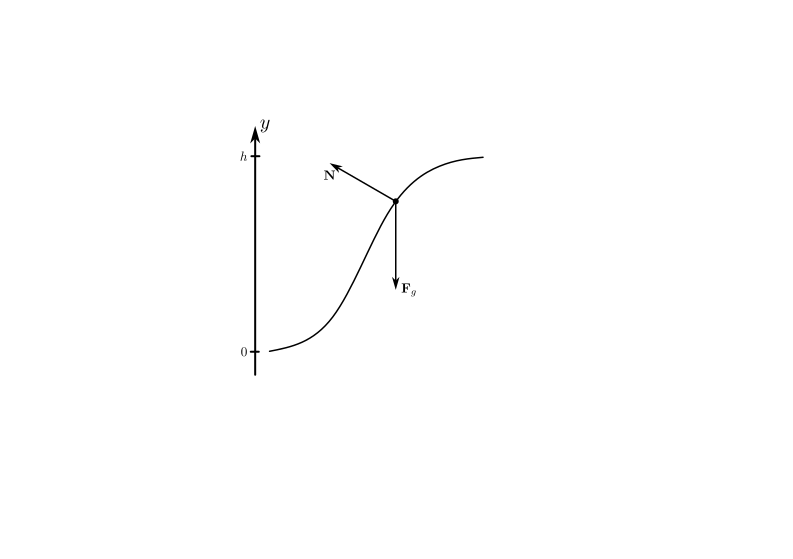
\includegraphics[scale=0.7]{../images/fig4_7.png}
    \caption{A threaded bead on a wire with two forces acting on it; The force of gravity $\vb{F}_g$
    is conservative and the normal force $\vb{N}$ is non-conservative.}
    \label{fig:4_7}
\end{figure}

(c) The bead is initially released from rest at a height $h$. From conservation of energy:
\begin{align}
    E_i &= E_f \\
    \frac{1}{3} m\gamma h^3 &= \frac{1}{2} m v^2 \\
    v &= \sqrt{\frac{2}{3} \gamma h^3}
\end{align}
where $v$ is the speed of the bead at the bottom of the wire.

\paragraph{4.9}
(a) Assuming the force of a one-dimensional spring $F = -kx$ is conservative, potential energy is
\begin{align*}
    U(x) = - \int_0^x F \dd{x'} = \frac{1}{2} kx^2  
\end{align*}
where $x$ is the displacement of the spring from its equilibrium position.

(b) From Newton's second law, the new equilibrium position $x_o$ is found when the spring force and
gravity are equal.
\begin{align*}
    0 = F + F_{g} = -kx_o + m g \implies x_o = \frac{mg}{k}
\end{align*}
When $y = 0$,  $U = 0$. Thus the potential energy is zero at position $x = x_o$:
\begin{align*}
    U(x_o) = \frac{1}{2} k(x_o)^2 - mg(x_o) = 0
\end{align*}
The total potential energy of the system at position $x = y + x_o$ is
\begin{align*}
    U(x) &= U_{sp} + U_{g} = \frac{1}{2} k(y+x_o)^2 - mg(y+x_o) \\
    &= \frac{1}{2} ky^2 + kyx_o - mgy + \frac{1}{2} kx_o^2 - mgx_o
\end{align*}
Since $kyx_o - mgy = 0$ and the last two terms are the potential energy at the new equilibrium
$U(x_o) = 0$, the total potential energy is $U(x) = \frac{1}{2} ky^2$.

\paragraph{4.11}
Finding the partial derivatives of the functions with constants $a,b,c$:

(a) $f(x,y,z) = ax^2 + bxy + cy^2$:
\begin{align*}
    \pdv{f}{x} &= 2ax + by \qquad \pdv{f}{y} = bx + 2cy \qquad \pdv{f}{z} = 0
\end{align*}

(b) $g(x,y,z) = \sin(axyz^2)$:
\begin{align*}
    \pdv{g}{x} &= ayz^2 \cos(axyz^2) \qquad \pdv{g}{y} = axz^2 \cos(axyz^2) 
    \qquad \pdv{g}{z} = 2axyz \cos(axyz^2)
\end{align*}

(c) $h(x,y,z) = ar$ where $r = \sqrt{x^2 + y^2 + z^2}$:
Since 
\begin{equation*}
    \pdv{r}{x_i} = \frac{x_i}{r}
\end{equation*}
The partial derivatives of $h$ are
\begin{align*}
    \pdv{h}{x} &= \frac{ax}{r} \qquad \pdv{h}{y} = \frac{ay}{r} \qquad \pdv{h}{z} = \frac{az}{r}
\end{align*}

\paragraph{4.13}
Calculating the gradient $\grad{f}$ of

(a) $f(x,y,z) = \ln(r) = \ln(\sqrt{x^2 + y^2 + z^2})$:
\begin{align*}
    \pdv{f}{x} &= \frac{x}{r^2} \qquad \pdv{f}{y} = \frac{y}{r^2}
        \qquad \pdv{f}{z} = \frac{z}{r^2} \\
    \grad{f} &= \frac{x}{r^2} \vu{x} + \frac{y}{r^2} \vu{y} + \frac{z}{r^2} \vu{z} 
    = \frac{\vu{r}}{r}
\end{align*}

(b) $f = r^n = (x^2 + y^2 + z^2)^{n/2}$ where $n$ is a constant:
\begin{align*}
    \pdv{f}{x} &= nr^{n-1} \frac{x}{r} = nr^{n-2} x \qquad \pdv{f}{y} = nr^{n-2} y
        \qquad \pdv{f}{z} = nr^{n-2} z \\
    \grad{f} &= nr^{n-2} x \vu{x} + nr^{n-2} y \vu{y} + nr^{n-2} z \vu{z} = nr^{n-1} \vu{r}
\end{align*}

(c) $f = g(r)$ where $g(r)$ is some unspecified function of $r$:
\begin{align*}
    \pdv{f}{x} &= g'(r) \pdv{r}{x} = g'(r) \frac{x}{r} \qquad 
    \pdv{f}{y} = g'(r) \frac{y}{r} \qquad \pdv{f}{z} = g'(r) \frac{z}{r} \\
    \grad{f} &= g'(r) \frac{x}{r} \vu{x} + g'(r) \frac{y}{r} \vu{y} + g'(r) \frac{z}{r} \vu{z}
    = g'(r) \vu{r}
\end{align*}

\paragraph{4.15}
Using the approximate formula for the change in $f$:
\begin{equation*} \tag{4.35}
    \dd{f} = \grad{f} \cdot \dd{\vb{r}}
\end{equation*}
For $f(\vb{r}) = x^2 + 2y^2 + 3z^2$, The approximation of moving from $\vb{r} = (1, 1, 1)$ to
$(1.01, 1.03, 1.05)$:
\begin{align*}
    \dd{f} &= \grad{f} \cdot \dd{\vb{r}} = (2x \vu{x} + 4y \vu{y} + 6z \vu{z}) \cdot 
    (0.01 \vu{x} + 0.03 \vu{y} + 0.05 \vu{z}) \\
    &= 0.02 + 0.12 + 0.30 = 0.44
\end{align*}
The exact change in $f$ is
\begin{align*}
    \Delta f = f(1.01, 1.03, 1.05) - f(1, 1, 1) = 0.4494
\end{align*}

\paragraph{4.17}
A charge $q$ experiences a constant force $\vb{F} = q \vb{E}_o$ where $\vb{E}_o$ is a uniform
electric field. 

(a) The work done by the force from point 1 to 2
\begin{align*}
    W = \int_1^2 \vb{F} \cdot \dd{\vb{r}} = q \vb{E}_o \cdot (\vb{r}_1 - \vb{r}_2)
\end{align*}
which is independent of the path hence it is a conservative force. Thus the potential energy is
\begin{equation*}
    U(\vb{r}) = - W(0 \to \vb{r}) = - q \vb{E}_o \cdot \vb{r}
\end{equation*}

(b) Checking that $\vb{F}$ is derivable from potential energy $U$:
\begin{align*}
    \vb{F} &= - \grad{U} = - \pdv{U}{x} \vu{x} - \pdv{U}{y} \vu{y} - \pdv{U}{z} \vu{z} \\
    &= - \pdv{x}(-q \vb{E}_o \cdot \vb{x}) \vu{x} - \pdv{y}(-q \vb{E}_o \cdot \vb{y}) \vu{y} 
    - \pdv{z}(-q \vb{E}_o \cdot \vb{z}) \vu{z} \\
    &= q \vb{E}_o (\vu{x} + \vu{y} + \vu{z}) = q \vb{E}_o
\end{align*}

\paragraph{4.18}
(a) If the vector $\grad{f}$ is perpendicular to the surface through $r$, then (4.35) becomes
\begin{equation}
    \dd{f} = \grad{f} \cdot \dd{\vb{r}} = 0
\end{equation}
since the dot product of perpendicular vectors is zero. Thus $f$ is constant on the surface.

(b) Choosing a small displacement $\dd{\vb{r}} = \epsilon \vb{u}$:
\begin{equation}
    \dd{f} = \grad{f} \cdot (\epsilon \vb{u}) = \epsilon \grad{f} \cdot \vb{u} 
        = \epsilon \abs{\grad{f}} \abs{\vb{u}} \cos \theta
\end{equation}
the corresponding maximum value of $\dd{f}$ is when $\theta = 0$ where $\vb{u}$ is in the same
direction as $\grad{f}$.

\paragraph{4.19}
(a) For a surface of constant $f$, $f = x^2 + 4y^2$ is an ellipse in the $xy$ plane cenetered at the
origin with semi-major axis $a = \sqrt{f}$ and semi-minor axis $b = \sqrt{f} / 2$. Since $z$ is
unspecified, the surface is an infinitely long elliptical cylinder.

(b) The gradient of $f$ is
\begin{align*}
    \grad{f} = 2x \vu{x} + 8y \vu{y}
\end{align*}
For a surface $f=5$ at the point $(1, 1, 1)$, the gradient is $\grad{f} = 2 \vu{x} + 8 \vu{y}$. From
Problem 4.18, $0 = \grad{f} \cdot \dd{\vb{r}}$ describes that $\grad{f}$ is normal to this surface.
Thus the unit normal vector is
\begin{align*}
    \vu{n} = \frac{\grad{f}}{\abs{\grad{f}}} = \frac{2 \vu{x} + 8 \vu{y}}{\sqrt{68}}
        = \frac{1 \vu{x} + 4 \vu{y}}{\sqrt{17}}
\end{align*}
or $-\vu{n}$ corresponding to the opposite direction. Moving along the direction of $\vb{n}$
maximizes the rate of change of $f$.

\paragraph{4.20}
Finding the curl, $\curl{\vb{F}}$, for the forces:

(a) $\vb{F} = k\vb{r}$
\begin{align*}
    \curl{k\vb{r}} &= \curl(kx \vu{x} + ky \vu{y} + kz \vu{z}) \\
    &= 0 \vu{x} + 0 \vu{y} + 0 \vu{z} = 0
\end{align*}

(b) $\vb{F} = (Ax, By^2, Cz^3)$ where $A,B,C$ are constants:
\begin{align*}
    \curl{(Ax, By^2, Cz^3)} = 0
\end{align*}

(c) $\vb{F} = (Ay^2, Bx, Cz)$:
\begin{align*}
    \curl{(Ay^2, Bx, Cz)} &= 
    \begin{vmatrix}
        \vu{x} & \vu{y} & \vu{z} \\
        \pdv{x} & \pdv{y} & \pdv{z} \\
        Ay^2 & Bx & Cz
    \end{vmatrix} \\
    &= (0) \vu{x} - (0) \vu{y} + (B - 2Ay) \vu{z} = (B - 2Ay) \vu{z}
\end{align*}

\paragraph{4.21}
Given the gravitational force
\begin{align*}
    \vb{F} = - \frac{GmM}{r^2} \vu{r} = - \frac{GmM}{r^3} \vb{r}
\end{align*}
The curl of $\vb{F}$ is
\begin{align*}
    \curl{\vb{F}} &= \curl{\frac{GmM}{r^3} \vb{r}} \\
    &= \frac{GmM}{r^3} \curl{\vb{r}} \\
    &= \frac{GmM}{r^3} \curl{(x \vu{x} + y \vu{y} + z \vu{z})} \\
    &= \frac{GmM}{r^3}
    \begin{vmatrix}
        \vu{x} & \vu{y} & \vu{z} \\
        \pdv{x} & \pdv{y} & \pdv{z} \\
        x & y & z
    \end{vmatrix} \\
    &= \frac{GmM}{r^3} (0 \vu{x} + 0 \vu{y} + 0 \vu{z}) = 0
\end{align*}
Thus the gravitational force is conservative. The potential energy is
\begin{align*}
    U(\vb{r}) = - \int_0^{\vb{r}} \vb{F} \cdot \dd{\vb{r}} = \frac{GmM}{r}
\end{align*}

\paragraph{4.23}
Find which of the following forces are conservative, and for those that are, find the potential and
verify that $\vb{F} = - \grad{U}$:

(a) $\vb{F} = k(x, 2y, 3z)$ where $k$ is a constant. The force is conservative when the curl is zero
\begin{align*}
    \curl{\vb{F}} = k \curl{(x, 2y, 3z)} = 0
\end{align*}
Thus the force is conservative and the potential energy is
\begin{align*}
    U(\vb{r}) = - \int_0^{\vb{r}} \vb{F} \cdot \dd{\vb{r}} = -\frac{1}{2} k(x^2 + 2y^2 + 3z^2)
\end{align*}
Verification of $\vb{F} = - \grad{U}$:
\begin{align*}
    -\grad{U} &= -\quantity(\pdv{U}{x}, \pdv{U}{y}, \pdv{U}{z}) \\
    &= k(x, 2y, 3z) = \vb{F}
\end{align*}

(b) $\vb{F} = k(y, x, 0)$: The curl of $\vb{F}$ is
\begin{align*}
    \curl{\vb{F}} = k \curl{(y, x, 0)} = 0
\end{align*}
Thus the force is conservative and the potential energy is
\begin{align*}
    U(\vb{r}) = - \int_0^{\vb{r}} \vb{F} \cdot \dd{\vb{r}}
    = -\int_0^{\vb{r}} F_x(x, 0) \dd{x'} + F_y(x, y) \dd{y'}
    = -k(xy)
\end{align*}
where the first integral is zero since $F_x = 0$. Differentiating the potential gives
\begin{align*}
    -\grad{U} = -\quantity(\pdv{x}(-kxy), \pdv{y}(-kxy)) = k(y, x) = \vb{F}
\end{align*}

(c) $\vb{F} = k(-y, x, 0)$: The curl of $\vb{F}$ is
\begin{align*}
    \curl{\vb{F}} = k \curl{(-y, x, 0)} = 2k \vu{z}
\end{align*}
Thus the force is not conservative.

\paragraph{4.25}
(a)
\begin{align*}
    \oint_\Gamma \vb{F} \cdot \dd{\vb{r}} &= \int_1^2 \vb{F} \cdot \dd{\vb{r}}
        + \int_2^1 \vb{F} \cdot \dd{\vb{r}} \\
    &= \int_1^1 \vb{F} \cdot \dd{\vb{r}} = 0
\end{align*}

(b)
If $\curl{\vb{F}} = 0$,
\begin{align*}
    \oint_\Gamma \vb{F} \cdot \dd{\vb{r}} &= \int \curl{\vb{F}} \cdot \vu{n} \dd{\vb{A}}
    = 0
\end{align*}

(c)
Integrating $\vb{F}$ around the closed path $\Gamma$:
\begin{align*}
    \oint_\Gamma \vb{F} \cdot \dd{\vb{r}} = &\int_B^{B+b} F_x(x, C, z) \dd{x}
        - \int_B^{B+b} F_x(x, C+c, z) \dd{x} \\
        &+ \int_C^{C+c} F_y(B+b, y, z) \dd{y} - \int_C^{C+c} F_y(B, y, z) \dd{y}
\end{align*}
where the first two terms are the path along the top and bottom of the rectangle and the last two
terms are the path along the left and right sides of the rectangle. Looking at the first two terms,
\begin{align*}
    -\int_B^{B+b} F_x(x, C+c, z) - F_x(x, C, z) \dd{x} 
    = -\int_B^{B+b} \int_C^{C+c} \pdv{F_x(x,y,z)}{y} \dd{y} \dd{x}
    = -\int_S \pdv{F_x}{y} \dd{A}
\end{align*}
The last two terms are
\begin{align*}
    \int_C^{C+c} F_y(B+b, y, z) - F_y(B, y, z) \dd{y} 
    = \int_C^{C+c} \int_B^{B+b} \pdv{F_y(x,y,z)}{x} \dd{x} \dd{y}
    = \int_S \pdv{F_y}{x} \dd{A}
\end{align*}
Hence the integral is
\begin{align*}
    \oint_\Gamma \vb{F} \cdot \dd{\vb{r}} = \int_S \pdv{F_y}{x} - \pdv{F_x}{y} \dd{A}
\end{align*}
where $\curl{\vb{F}} = \pdv{F_y}{x} - \pdv{F_x}{y}$. Thus
\begin{align*}
    \oint_\Gamma \vb{F} \cdot \dd{\vb{r}} = \int_S \curl{\vb{F}} \cdot \vu{n} \dd{A}
\end{align*}

\paragraph{4.27}
From the time-dependent PE for any fixed time $t$
\begin{equation*} \tag{4.48}
    U(\vb{r}, t) = -\int_{\vb{r}_o}^{\vb{r}} \vb{F}(\vb{r}', t) \cdot \dd{\vb{r}'}
\end{equation*}
and the force as a gradient of PE:
\begin{align*}
    -\grad{U}(\vb{r}, t) &= \pdv{U}{r} \int \vb{F}(\vb{r}', t) \cdot \dd{\vb{r}'}
        + \pdv{U}{t} \int \vb{F}(\vb{r}', t) \cdot \dd{\vb{r}'} \\
\end{align*}
Since $t$ is fixed, and by the fundamental theorem of calculus
\begin{align*}
    -\grad{U}(\vb{r}, t) = \vb{F}(\vb{r}, t)
\end{align*}
For closer inspection, the change in $U$ from a small displacement $\dd{\vb{r}}$  and 
\begin{align*}
    \dd{U} = U(\vb{r} + \dd{\vb{r}}, t + \dd{t}) - U(\vb{r}, t)
\end{align*}
rewritten as partial derivatives
\begin{align*}
    \dd{U} = \grad{U} \cdot \dd{\vb{r}} + \pdv{U}{t} \dd{t}
\end{align*}
Given the force is conservative $\vb{F} = -\grad{U}$ and the change in $T$ is defined as
$\dd{T} = \vb{F} \cdot \dd{\vb{r}}$ the work done by the force in the displacement $\dd{\vb{r}}$:
\begin{align*}
    \dd{U} &= -\dd{T} + \pdv{U}{t} \dd{t} \\
    \dd(U + T) &= \pdv{U}{t} \dd{t}
\end{align*}
Hence, the total mechanical energy is conserved only when $\pdv*{U}{t} = 0$ and false otherwise.

\paragraph{4.28}
(a) From conservation of energy, the total mechanical energy is
\begin{align*}
    E = T + U = \frac{1}{2} m \dot{x}^2 + \frac{1}{2} k x^2
\end{align*}
Solving for velocity $\dot{x}$:
\begin{align*}
    \dot{x} = \pm \sqrt{\frac{2}{m} \quantity(E - \frac{1}{2} k x^2)}
\end{align*}
(b) At the spring's max displacement $x_{max} = A$, the kinetic energy is zero hence a total energy
\begin{align*}
    E = U = \frac{1}{2} k A^2
\end{align*}
subbing into the equation for velocity
\begin{align*}
    \dot{x} = \pm \sqrt{\frac{2}{m} \quantity(\frac{1}{2} k A^2 - \frac{1}{2} k x^2)}
    = \pm \sqrt{\frac{k}{m} \quantity(A^2 - x^2)}
\end{align*}
Solving for the time to go from the origin $x=0$ at time $t=0$ to a position $x$:
\begin{align*}
    t = \int_0^t \dd{t} = \int_0^x \frac{\dd{x'}}{\dot{x}(x')} 
    = \sqrt{\frac{m}{k}} \int_0^x \frac{\dd{x'}}{\sqrt{(A^2 - x'^2)}}
    = \sqrt{\frac{m}{k}} \arcsin(\frac{x}{A})
\end{align*}
Solving $x$ as a function of $t$:
\begin{align*}
    x = A \sin(\sqrt{\frac{k}{m}} t)
\end{align*}
where the function $\sin(\omega t)$ has a period $T = 2\pi / \omega = 2\pi \sqrt{m/k}$.
\end{document}